\subsection{Preliminary experiments: encoding hierarchical rules}
Before diving into the FET task, KENN has been tested in a hierarchical classification scenario. Since the goal of this preliminary phase is to familiarize with KENN rather than achieve the best performance, we do not dwell on the architecture, training setup, and results. We focus, instead, on how hierarchical relations can be encoded with KENN. Different heuristics to represent a hierarchy through logical rules are proposed within these preliminary studies.

\subsubsection{Dataset}
% The baseline model implemented for these experiments has a simple architecture. It uses DistilBERT as encoder, followed by a dense fully connected layer and a final classification layer that applies the sigmoid activation function. The choice of this activation function is due to the fact that in a multilabel task we want as output the probability of each label. Starting from this architecture, KENN is placed between the fully connected layer and the classification layer. Clause weights are set as learnable parameters with an initial value of 0.5.

The dataset used for this experiment is called DBpedia Classes\footnote{https://www.kaggle.com/danofer/dbpedia-classes}. It is composed of approximately 240k labeled Wikipedia articles, where the only feature is the span of text. The types are organized as a forest of 9 trees, each of them representing a 3-level hierarchy. The type set counts 298 types: 9 at top-level, 70 at middle-level, and 219 at low-level. Each example is labeled with exactly 3 classes from the full path of a tree (i.e., one class per level). For example, if we consider the \textit{Species} tree shown in Figure~\ref{fig:dbpedia_classes}, an instance of the dataset could present $ label_{1} = Species $, $ label{_2} = Animal $, and $ label_{3} = Bird $.

\begin{figure}[H]
    \centering
    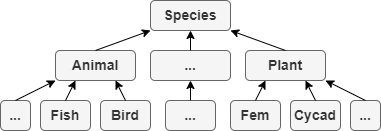
\includegraphics[width=.7\linewidth]{dbpedia_classes.png}
    \caption{Example of a tree of DBpedia Classes}
    \label{fig:dbpedia_classes}
\end{figure}

\subsubsection{Knowledge definition} \label{knowledge_generation}
The first step to integrate KENN is to create the logical KB. We can start from the tree in Figure~\ref{fig:dbpedia_classes} and then generalize different strategies for defining logical rules. The most intuitive and straightforward way consists in following the \textit{is-a} relations, which are implicitly encoded in the tree structure. Considering the picture, it is possible to state that if an instance is a \texttt{Fish}, then it is an \texttt{Animal}. In the same way, we can then proceed with the next level of the hierarchy and state that if an instance is an \texttt{Animal}, then it is a \texttt{Species}. This mechanism can be extended to all the other subtrees to create a logical clause per edge. The resulting KB will be a set of logical implications between subtypes and supertypes. Even if it seems a natural way to describe the hierarchy, it doesn't necessarily mean it is the most effective solution. For this reason, we should take a step back and analyze the alternatives offered by the hierarchy. Figure~\ref{fig:hierarchy_example} shows a generic hierarchy and highlights two groups of constraints we can distinguish:
\begin{enumerate}
    \item \textbf{Vertical constraints:} based on the paths of a tree, they can be used to represent specialization relations
    \item \textbf{Horizontal constraints:} based on pairs of nodes from different branches, they can be used to represent disjointness relations
\end{enumerate}
\begin{figure}[H]
    \centering
    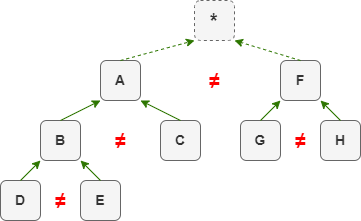
\includegraphics[width=.7\linewidth]{hierarchy_example.png}
    \caption{Examples of a generic hierarchy. In green the vertical constraints, in red the horizontal constraints.}
    \label{fig:hierarchy_example}
\end{figure}
For each group of constraints, it is possible to implement different strategies to define the KB. In the rest of the thesis, these strategies will be referred to as \textit{KB modes}. Note that in the definitions below we will use unary predicates to represent the belonging of an instance $X$ to a type.

\paragraphn{Vertical Constraints}
Using the unary predicates $Subtype$ and $Supertype$ such that the type $Subtype$ is a specialization of the type $Supertype$, we can define three main strategies to build vertical constraints:
\begin{itemize}
    \item \textbf{Bottom Up:}
        \begin{itemize}
            \item FOL: $ \forall X, Subtype(X) \to Supertype(X) $
            \item KENN: $ \neg Subtype \vee Supertype $
            \item Defined by following every path of the tree from the leaves to the root. It represents the logic dependency between types, following the most widely used semantics in the definition of subclass.
            \item Open World Assumption: a clause is satisfied even when an instance is assigned only to supertypes
        \end{itemize}
    \item \textbf{Top Down:}
        \begin{itemize}
            \item FOL: $ \forall X, Supertype(X) \to (Subtype_{1}(X) \vee ... \vee Subtype_{n}(X)) $
            \item KENN: $ \neg Supertype \vee Subtype_{1} \vee ... \vee Subtype_{n}  $
            \item Defined by following every path of the tree from the root to the leaves
            \item Closed World Assumption: a clause is not satisfied when an instance is assigned to a supertype without any of its subtypes
        \end{itemize}  
    \item \textbf{Hybrid:} 
    \begin{itemize}
        \item Composed of a mix of \textit{Bottom Up} and \textit{Top Down} clauses
    \end{itemize}
\end{itemize}
Note that if a model that uses this kind of knowledge is confident about a given type, a \textit{Bottom Up} clause propagates this certainty towards the root of the hierarchy. Conversely, a \textit{Top Down} clause only guarantees that one of the subtypes is appropriate, but provides no information as to which one. The reason, of course, is the tree-like hierarchy, where each type has only one parent, but potentially many descendants.

The presented KB modes can be considered as the starting point to create new strategies by adding some variations. In Table~\ref{tab:kb_modes} we can find a summary that comprehends every KB mode, each of them accompanied by examples of clauses from the hierarchy in Figure~\ref{fig:dbpedia_classes}. Before proceeding with the explanation of the variants, we have to make clear why they have been introduced: the conflicts. If we look at the table, we can see that in the examples of the pure \textit{Bottom Up} and \textit{Top Down} modes there are conflicts: a middle-level label appears both as positive and negative literal. This fact derives from the translation of the logical implication into a disjunction since an intermediate node is at the same time antecedent and consequent of different logical implications. This behavior still hold for the \textit{Hybrid} mode.

Now that the possible problems of the starting strategies are known, it is possible to introduce their conflict-free variants. These variants avoid conflict situations in different ways. The ``Skip" ones rely on the transitivity of a relation by linking top-level and low-level nodes by skipping those middle-level nodes that would create a conflict (i.e., a middle-level node cannot be the antecedent of an implication rule). These solutions provide a more shallow representation of the knowledge, especially for the \textit{Top Down Skip}. In this case, a logical rule that represents the relation between top-level and low-level lose effectiveness because the implication may have too many consequents. The \textit{Hybrid In} and \textit{Hybrid Out} modes, instead, avoid conflicts by fixing the middle-level types as consequent or antecedent of an implication rule, respectively. In this way, the deltas produced by each CE for the same literal will always have the same sign.

Note that the proposed variants are valid for this dataset, but some of them do not apply to every context since they require a hierarchy with at least 3 levels.

\begin{table}
\centering
\caption{Strategies for defining logical clauses based on the hierarchy in Figure~\ref{fig:dbpedia_classes}}
\label{tab:kb_modes}
\begin{tabular}{c|l|}
\cline{2-2}
                                              & \multicolumn{1}{c|}{\textbf{Clauses}}                                                                                                                                                                                             \\ \hline
\multicolumn{1}{|c|}{\textbf{Bottom Up}}      & \begin{tabular}[c]{@{}l@{}}$ c_{1}: \neg Fish \vee Animal $\\ $ c_{2}: \neg Bird \vee Animal $\\ $ c_{3}: \neg Animal \vee Species $\\ ...\end{tabular}                                                                           \\ \hline
\multicolumn{1}{|c|}{\textbf{Top Down}}       & \begin{tabular}[c]{@{}l@{}}$ c_{1}: \neg Species \vee Animal \vee ... \vee Plant $\\ $ c_{2}: \neg Animal \vee Fish \vee ... \vee Bird $\\ $ c_{3}: \neg Plant \vee Fem \vee ... \vee Cycad $\\ ...\end{tabular}                  \\ \hline
\multicolumn{1}{|c|}{\textbf{Hybrid}}         & \begin{tabular}[c]{@{}l@{}}$ c_{1}: \neg Species \vee Animal \vee ... \vee Plant $\\ $ c_{2}: \neg Animal \vee Species $\\ $ c_{3}: \neg Plant \vee Species $\\ ...\end{tabular}                                                  \\ \hline
\multicolumn{1}{|c|}{\textbf{Bottom Up Skip}} & \begin{tabular}[c]{@{}l@{}}$ c_{1}: \neg Fish \vee Animal $\\ $ c_{2}: \neg Fish \vee Species $\\ $ c_{3}: \neg Bird \vee Animal $\\ $ c_{4}: \neg Bird \vee Species $\\ ...\end{tabular}                                         \\ \hline
\multicolumn{1}{|c|}{\textbf{Top Down Skip}}  & \begin{tabular}[c]{@{}l@{}}$ c_{1}: \neg Species \vee Animal \vee ... \vee Plant $\\ $ c_{2}: \neg Species \vee Fish \vee ... \vee Bird \vee Fem \vee Cycad $\\ ...\end{tabular}                                                  \\ \hline
\multicolumn{1}{|c|}{\textbf{Hybrid In}}      & \begin{tabular}[c]{@{}l@{}}$ c_{1}: \neg Species \vee Animal \vee ... \vee Plant $\\ $ c_{2}: \neg Fish \vee Animal $\\ $ c_{3}: \neg Bird \vee Animal $\\ $ c_{4}: \neg Fem \vee Plant $\\ ...\end{tabular}                      \\ \hline
\multicolumn{1}{|c|}{\textbf{Hybrid Out}}     & \begin{tabular}[c]{@{}l@{}}$ c_{1}: \neg Animal \vee Species $\\ $ c_{2}: \neg Animal \vee Fish \vee ... \vee Bird $\\ $ c_{3}: \neg Plant \vee Species $\\ $ c_{4}: \neg Plant \vee Fem \vee ... \vee Cycad $\\ ...\end{tabular} \\ \hline
\end{tabular}
\end{table}

\paragraphn{Horizontal Constraints}
These constraints aim to avoid the co-occurrence of types whose instances form disjoint sets (e.g., if an example is labeled as \texttt{Person} it cannot be labeled as \texttt{Location} and vice versa). Using $T_i$ to indicate an arbitrary type, the logical rule that best represents this constraint is:
\begin{gather*}
    \forall X, T_{1}(X) \to (\neg T_{2}(X) \wedge ... \wedge \neg T_{n}(X))
\end{gather*}
With the following steps, we can derive an equivalent formula without implication and conjunctions:
\begin{align*}
    & T_{1} \to (\neg T_{2} \wedge ... \wedge \neg T_{n}) = \\
    & = \neg T_{1} \vee (\neg T_{2} \wedge ... \wedge \neg T_{n}) = \\
    & = \neg T_{1} \vee \neg (T_{2} \vee ... \vee T_{n})
\end{align*}
Unfortunately, the derived formula cannot be furthermore decomposed due to the presence of parentheses. We can opt for two alternative solutions to bypass the problem:
\begin{enumerate}
    \item \textbf{Approximate the rule with a softer constraint:} if an instance does not belong to \texttt{T$_1$}, then it should belong to another type. \\
    The logical formula for this statement is:
    \begin{gather*}
            \forall X, \neg T_{1}(X) \to (T_{2}(X) \vee ... \vee T_{n}(X))
    \end{gather*}
    that can be translated into KENN's language with the following steps:
    \begin{align*}
        & \neg T_{1} \to (T_{2} \vee ... \vee T_{n}) = \\
        & = T_{1} \vee (T_{2} \vee ... \vee T_{n}) = \\
        & = T_{1} \vee T_{2} \vee ... \vee T_{n}
    \end{align*}
    From a logical point of view, the resulting formula does not seem very helpful because it simply states that an instance belongs at least to one class. Indeed, if we repeat the previous steps using any other type as the antecedent of the implication, the derived clause will be identical. Furthermore, the action of KENN on such clauses would not lead to mutual exclusivity because every literal is positive and none of the involved predictions will receive a negative boost.
    
    \item \textbf{Split the rule into multiple clauses:} define a clause for each pair of disjoint types.
    Given two disjoint types, the logical formula to express the mutual exclusivity is:
    \begin{gather*}
        \forall X, T_{1}(X) \to \neg T_{2}(X)
    \end{gather*}
    If we consider $n$ disjoint pairs in which appears $T_{1}$, the resulting KB in KENN's language will be the following:
    \begin{align*}
        & c_{1}: \neg T_{1} \vee \neg T_{2}\\
        & ...\\
        & c_{n}: \neg T_{1} \vee \neg T_{n}
    \end{align*}
    Unlike strategy 1, this one preserves the soundness of the starting formula. However, there are still some issues to take into account. The first concerns the number of clauses necessary to cover the possible combinations of pairs: having $ n $ mutual independent types will result in $ \frac{n!}{2!(n-2)!} $ logical clauses. The second issue regards the action of KENN: while in strategy 1 there were only positive literals, in this strategy there are only negative literals, thus meaning that none of the predictions will ever receive a positive boost.
\end{enumerate}

\paragraphn{Horizontal constraints - Alternative usage}
Another use of horizontal constraints that is not related to this dataset, but could be useful in other contexts, is to encourage the co-occurrence between different types. Here the purpose is exactly the opposite with respect to the previous rules. Even if this goal can be reached by applying a simple inference on the final predictions without the use of KENN, in some tasks (e.g., domain adaptation) it may be useful to leave the decision to the network. If we want the model to learn a mapping between two types \texttt{A} and \texttt{B}, we can define the logical rule
\begin{gather*}
    (A \to B) \wedge (B \to A)
\end{gather*}
that can be expressed in KENN using the following clauses:
\begin{align*}
    & c1: \neg A \vee B \\
    & c2: \neg B \vee A
\end{align*}
The first thing we can notice is the presence of conflicts, but they will not have a negative impact on the final predictions. The preactivation of the literals belonging to the two clauses are the same with opposite signs, so a  literal cannot be dominant in both clauses. In other words, the final predictions always benefit from the knowledge enhancement since the effect of KENN will be one of the following:
\begin{itemize}
    \item \textbf{positive preactivations:} a positive aggregated delta is produced for each literal
    \item \textbf{negative preactivations:} a negative aggregated delta is produced for each literal
    \item \textbf{discord preactivations:} an aggregated delta with the sign of the highest\footnote{in absolute value} preactivation is produced for each literal
\end{itemize}


\subsubsection{Results}
As anticipated, the results are not the focus of this study since we are not dealing with the target problem of this thesis. To see KENN in action, the KB modes of Bottom Up, Top Down, Hybrid In, and Hybrid Out have been evaluated. 
The baseline model implemented for these experiments has a simple architecture. It uses DistilBERT as encoder, followed by a dense fully connected layer and a final classification layer that applies the sigmoid activation function. The choice of this activation function is due to the fact that in a multilabel task we want as output the probability of each label. Starting from this architecture, KENN is placed between the fully connected layer and the classification layer. Clause weights are set as learnable parameters with an initial value of 0.5.

In Table \ref{tab:performance_dbpedia} are reported the results obtained by the baseline and KENN-based models. Hybrid Out is the configuration that brought more benefits to the baseline model with a $+0.0157$ on the F1 score, thanks to its highest recall. Even Top Down brought improvements with an increase of $+0.0097$. This did not happen with the other configurations.

An interesting fact that emerged regards the clause weights. By inspecting the final weights learned by the models, it was found out that the models that performed the best are the ones that finished the train with higher clause weights. In particular, some clauses have increased their starting weight by 10 times. On the contrary, the worst models are the ones whose final weights are smaller. This fact means that KENN helped the baseline model the most when it gained more influence on the final predictions. From these results, we can say that the higher the weight, the better the performance. This result may lead to think that it could be reasonable to set higher initial clause weights to anticipate the learning process. However, we have to take this conclusion with a grain of salt because it could be strictly related to this dataset.

\begin{table}[H]
\centering
\caption{Comparison between the baseline and KENN-based models on DBpedia Classes in terms of \textit{macro f1 classes}}
\label{tab:performance_dbpedia}
\begin{tabular}{|c|ccc|}
\hline
\textbf{KB mode} & \multicolumn{1}{c|}{\textbf{P}} & \multicolumn{1}{c|}{\textbf{R}} & \textbf{F1}     \\ \hline
- (baseline)       & 0.9265                          & 0.8644                          & 0.8897          \\ \hline
Bottom Up      & 0.924                           & 0.8685                          & 0.8901          \\ \hline
Top Down       & \textbf{0.93}                   & 0.8788                          & 0.8994          \\ \hline
Hybrid In      & 0.9186                          & 0.87                            & 0.8884          \\ \hline
Hybrid Out     & 0.927                           & \textbf{0.8913}                 & \textbf{0.9054} \\ \hline
\end{tabular}
\end{table}